\section{Aufbau}
\label{sec:Aufbau}
%\begin{figure}
%	\centering
%	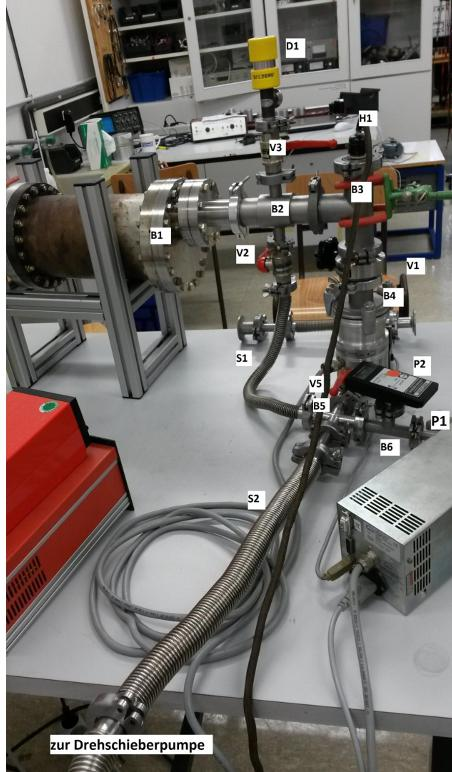
\includegraphics[width=\linewidth-70pt,height=\textheight-70pt,keepaspectratio]{content/images/Aufbau.eps}
%	\caption{Schematischer Aufbau zur Bestimmung des Elastizitätsmoduls\cite{V103}}
%	\label{fig:Aufbau}
%\end{figure}
Wie in Abbildung \ref{fig:Aufbau} zu sehen, kann der Stab entweder mit der Spannvorrichtung $C$ auf der einen Seite eingespannt oder auf den Auflagepunkten $A$ und $B$ auf beiden Seiten gelagert werden.
Zur Bestimmung der Durchbiegung sind verschiebbar an einer horizontalen Skala Messuhren mit Taststift angebracht.
